\cotefile{63}
\scanpage{41}
\noindent\hfill atkin \mspage{1}\margin{\handwritten{\illegible{1}\figure{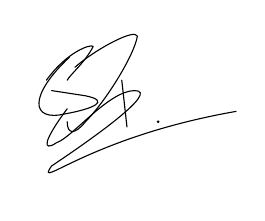
\begin{tikzpicture}[x=.33mm,y=-.33mm,line cap=round,line join=round]
\draw (4,18) .. controls (12,7) and (21,4) .. (22,5) .. controls (19,11) and (13,16) .. (12,18);
\draw (15,13) .. controls (23,6) and (38,-2) .. (39,1) .. controls (38,8) and (27,26) .. (19,34) .. controls (15,39) and (12,39) .. (12,34);
\draw (13,9) .. controls (-3,24) and (-2,34) .. (11,31) .. controls (22,29) and (29,26) .. (19,24) -- (6,22);
\draw (12,29) .. controls (3,41) and (2,46) .. (8,42) .. controls (14,40) and (28,22) .. (38,22) .. controls (48,22) and (21,41) .. (6,51) .. controls (-1,61) and (20,40) .. (77,30);
\draw (33,18) -- (35,36);
\fill (47,34) circle (.55);
\end{tikzpicture}}}}

\begin{center}
CONGRUENCES FOR MODULAR FORMS\quad \handwritten{(1968)}

by

A.O.L.ATKIN*
\end{center}

\handwritten{\figure{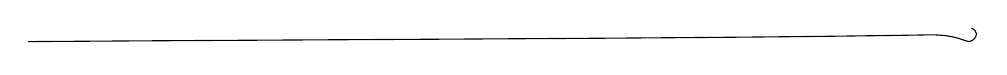
\begin{tikzpicture}[x=\linewidth,y=1mm,line cap=round]
\draw (0,0) .. controls (.35,.3) and (.72,.4) .. (.94,.85) .. controls (.98,1) and (.982,-.55) .. (.99,.25) .. controls (.994,.65) and (.995,1.35) .. (.988,1.7);
\end{tikzpicture}}}

\noindent * Research Fellow of the Atlas Computer Laboratory

\handwritten{\figure{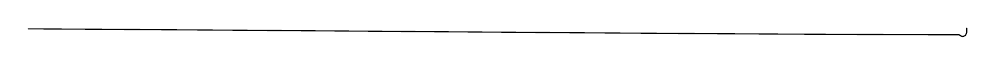
\begin{tikzpicture}[x=\linewidth,y=1mm,line cap=round]
\draw (0,.3) .. controls (.32,.08) and (.72,-.4) .. (.975,-.45) .. controls (.981,-1.05) and (.984,-.36) .. (.983,.38);
\end{tikzpicture}}}

\noindent 1. Introduction. This paper describes in general terms my attempts to extend and generalise congruence properties of modular forms with the aid of a computer(the ICT Atlas 1 computer of the Science Reserach Council at Chilton). The main practical conclusion can be stated simply: working in continuous direct contact with a large and powerful computer establishment has led to results far beyond my original expectations. Accordingly it seems worth while to try and give here some account of the actual process of discovery as it appeared to me at the time,which involves in effect a description of the work in reverse logical order; and to publish elsewhere the full mathematical details and a ``logical'' exposition based on the work in reverse order of time.

I have used Atlas to obtain a number of results,some of which are more interesting computationally than the present work. But in so far as the computer's function is to assist research,what matters is the final mathematical result rather than(to be fanciful) the machine's personal enjoyment of the tasks it has been ordered to perform. I am perfectly clear that the work described in this paper represents the most significant use I have made of Atlas. It might in theory have been possible to arrive at some of these results by \uline{a priori} reasoning; certainly the \unsure{.}cases where the proofs are complete require in the event no more computation than a few hours' hand work. But I would not myself have been able to conjecture the possibility of such results without the evidence provided by the computer.

I should like to thank the Director,Dr. J.Howlett,and my other colleagues at the Atlas Computer Laboratory for the frequent help they have given me. In particular I have had many valuable discussions

% archive sheet number: 40

\scanpage{42}
\noindent\hfill atkin \mspage{2}

\noindent with Dr. R.F.Churchhouse,both a number theorist and a veteran programmer,and Mr. \handwritten{E}.B.Fossey and Miss Barbara Stokoe have constantly assisted me with the Atlas Hartran(Fortran) system.

It is intended that this account shall be intelligible to the reader with no knowledge of modular theory\S{}\inserted{\handwritten{,}}\margin{\handwritten{\unsure{\S|$\delta$}/\ (comma)}}provided that he is prepared to accept that the coefficient \uline{$c(n)$} which we mainly consider is mathematically significant. However at some points we give brief additional explanations for the reader who has such knowledge.

\noindent\margin{\handwritten{/}}2. \uline{Ramanujan} \deleted{C}\uline{ongruences} \uline{for} \uline{primes} $q\handwritten{\leq}11$. The general theory of elliptic and modular functions had been in the process of development for about a century before RAMANUJAN(1919)conjectured his remarkable congruences for the partition function \uline{$p(n)$},defined combinatorially as the number of distinct ways of expressing \uline{$n$} as the sum of integral parts,where the order of the parts is immaterial. His conjecture was
\[
\handwritten{\text{\uline{if}}\quad 24n-1\equiv0\;(\text{\uline{mod}}\;5^{a}7^{b}11^{c})\quad
\text{\uline{then}}\quad p(n)\equiv0\;(\text{\uline{mod}}\;5^{a}7^{b}11^{c})}
\tag*{\handwritten{$\ldots$ (2.1)}}
\]
The curious appearance of $24n-1$ in \handwritten{(2.1)} is due to the fact that, writing
\[
\begin{aligned}
&\handwritten{x=e^{2\pi i\tau}\qquad (\,|x|<1,\ \mathrm{Im}\,\tau>0),}\\
&\handwritten{f(x)=(1-x)(1-x^{2})(1-x^{3})\ldots,}\\
\text{\deleted{we have}}\quad &\handwritten{\eta(\tau)=e^{\pi i\tau/12}f(x),}\\
\text{\inserted{\handwritten{we have}}}\quad &\handwritten{\sum_{n=0}^{\infty}p(n)\,x^{n}=1/f(x),}
\end{aligned}
\tag*{\handwritten{(2.2)}}
\]
and $\handwritten{\eta(\tau)}$ is a modular form of half-integral dimension and complicated multiplier system. Thus the congruence properties are naturally associated not with \uline{$f(x)$} whose reciprocal enumerates \uline{$p(n)$},but with \uline{$x^{1/24}f(x)$} ; that is,they are essentially modular and not combinatorial.$^{*}$ Ramanujan himself was of course well aware of this,

\noindent\handwritten{\rule{\linewidth}{0.4pt}}

\noindent\deleted{as his proofs}

\noindent *But see DYSON(19\handwritten{44}) and ATKIN and SWINNERTON-DYER(1954)for an exception.

\noindent\handwritten{\rule{\linewidth}{0.4pt}}

\noindent as his proofs of some particular cases show.

However this conjecture \handwritten{(2.1)},originally found from the

% archive sheet number: 41

\scanpage{43}
\noindent\hfill \unsure{a}\illegible{1}n \mspage{3}

\noindent evidence of hand computed tables,was found to fail for the case of $7^{3}$ by CHOWLA(1934) who observed that $p(243)$,computed by GUPTA(1935), is not divisible by $7^{3}$. This provides a simple illustration of the value of computers; had Ramanujan lived 50 years later he would surely have tested his conjecture extensively and probably found the correct form for $7$. WATSON(1938)proved the conjecture for all powers of $5$,and a suitably modified form for all powers of $7$,while ATKIN(1967)proved the conjecture for all powers of $11$. Thus the true form of \handwritten{(2.1)} is
\[
\begin{aligned}
&\handwritten{\text{\uline{if}}\quad 24n-1\equiv0\,(\text{\uline{mod}}\;5^{a}7^{b}11^{c})\quad
\text{\uline{then}}\quad p(n)\equiv0\,(\text{\uline{mod}}\;5^{a}7^{\beta}11^{c}),}\\
&\qquad\handwritten{\text{\uline{where}}\quad \beta=[(b+2)/2].}
\end{aligned}
\tag*{\handwritten{(2.3)}}
\]

It might be argued that for Ramanujan to have obtained the correct form \handwritten{(2.3)}would have been relatively unimportant; that the \uline{idea} of such a prop\rlap{\handwritten{\tikz[baseline=0pt,x=.7em,y=1ex,line cap=round]{\draw (-.18,-.82)--(.04,-.20)--(.45,-.78);\draw (.04,.4)--(.32,1.75);}}}\inserted{\handwritten{\uline{e}}}\margin{\handwritten{\tikz[x=.32em,y=.72ex,line cap=round]{\draw (0,0)--(1.2,3.4);\draw (.25,.68).. controls (.6,1.0) and (.8,.1) ..(1.2,.1);}}}rty is all that matters short of actual proof. But this is far from true in this kind of work,since the exact numerical form of such results can often provi\rlap{\handwritten{\tikz[baseline=0pt,x=1em,y=1ex]{\draw (0,-.35)--(.56,-.35)--(.56,1.7)--(1.06,1.7);}}}ed important clues as to a possible method of proof.

Despite the early recognition of the modular nature o\deleted{\unsure{n|f}}\handwritten{f} these congruences,it was not until 1949 that LEHNER(1949a,1949b) considered the analogous properties of $c(n)$,where
\[
\handwritten{j(\tau)=j(x)=\sum_{n=-1}^{\infty}\unsure{c|C}(n)\,x^{n}
=\left\{1+240\sum_{n=1}^{\infty}\sigma_{3}(n)x^{n}\right\}^{3}\big/xf^{24}(x)-744^{*}}
\tag*{\handwritten{$\ldots$ (2.4)}}
\]

\noindent\handwritten{\rule{\linewidth}{0.4pt}}

\noindent *We choose the arbitrary constant in $j(x)$ to make $c(0)=0$ and thus avoid tiresome exceptions to our results.

\handwritten{\figure{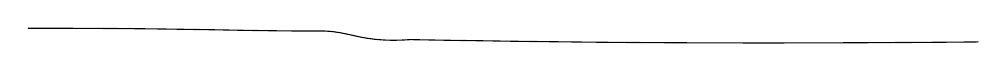
\begin{tikzpicture}[x=\linewidth,y=1mm,line cap=round]
\draw (0,.5) .. controls (.18,.5) and (.23,.1) .. (.31,.15) .. controls (.34,0) and (.35,-1.35) .. (.4,-.95) .. controls (.55,-1.25) and (.71,-1.55) .. (.995,-1.24);
\end{tikzpicture}}}

\[
\handwritten{\text{and}\qquad \sigma_{3}(n)=\sum_{d\mid n}d^{3}.}
\]

This function $j(\handwritten{\tau})$ is essentially the simplest of all modular forms, being in fact the Hauptmodul of the full modular group so that
\[
\handwritten{j\left(\frac{a\tau+b}{c\tau+d}\right)=j(\tau)\quad
\text{\uline{for} \uline{all} \uline{integral}}\quad a,b,c,d\quad
\text{\uline{with}}\quad ad-bc=1.}
\]
The results for $c(n)$ are
\[
\begin{aligned}
&\handwritten{\text{if}\quad n\equiv0\,(\mathrm{mod}\;2^{a}3^{b}5^{c}7^{d}11^{e})\quad
\text{then}\quad c(n)\equiv0\,(\mathrm{mod}\;2^{3a+8}3^{2b+3}\,\unsure{<|\hookleftarrow}}\\
&\hspace{4em}\handwritten{\unsure{>|\hookrightarrow}\,5^{c+1}7^{d}11^{e}).}
\end{aligned}
\tag*{\handwritten{(2.5)}}
\]

% archive sheet number: 42

\scanpage{44}
\noindent\hfill atkin \mspage{4}

\noindent These are all due to LEHNER(1949a,1949b,1950) except the cases \uline{$e$}$\handwritten{>}3$ due to ATKIN(1967). They represent what are perhaps the simplest and most natural ``Ramanujan-type'' congruences. The general possibilities are not confined to the coefficients \uline{$c(n)$} and \uline{$p(n)$},and many other modular forms have Fourier coefficients* with similar p\rlap{\handwritten{\tikz[baseline=0pt,x=1em,y=1ex]{\draw (0,-.35)--(.56,-.35)--(.56,1.7)--(1.06,1.7);}}}orperties. The work

\noindent\handwritten{\rule{\linewidth}{0.4pt}}

\noindent *That is,the coefficients of the expansion of a form $F(\handwritten{\tau})$ in powers of $x=\handwritten{e^{2\pi i\tau}}$.

\noindent\handwritten{\rule{\linewidth}{0.4pt}}

\noindent described in this paper was in fact conducted simultaneously with \uline{$c(n)$} and \uline{$p(n)$},the former being the simplest case and the latter an example\unsure{.} of the most difficult type of case; but we confine ourselves to \uline{$c(n)$} from now on in the present account.

\noindent 3. \uline{Congruences} \uline{for} $q=13$. It might have been hoped that results similar to \handwritten{(2.5)} would exist for primes $q\handwritten{>}11$,but this is(by now)extremely improbable(there are strong theoretical grounds for this assertion which is not merely based on the fact that no properties have been found).

\noindent The first results for $q\handwritten{>}11$,of an entirely different kind from those described in \handwritten{\S}2,are due to NEWMAN(1958),who proved that
\[
\handwritten{\unsure{c|C}(13^{2}n)\equiv8\,c(13n)\quad(\mathrm{mod}\;13),}
\tag*{\handwritten{(3.1)}}
\]
\[
\begin{aligned}
&\handwritten{\text{and}\quad\text{if}\quad t(n)=-c(13n)\quad\text{and}\quad p\ne13\quad\text{is prime then}}\\
&\qquad\handwritten{t(np)-t(n)t(p)+p^{11}\,t(n/p)\equiv0\,(\mathrm{mod}\;13).}
\end{aligned}
\tag*{\handwritten{$(3.2)^{*}$}}
\]

\noindent\handwritten{\rule{\linewidth}{0.4pt}}

\noindent *For any number-theoretic coefficient \uline{$t(n)$} we write $t(n)=0$ if \uline{$n$} is not an integer.

\noindent\handwritten{\rule{\linewidth}{0.4pt}}

From these Newman deduces,using the computed ``accident'' that $c(7\mathbin{.}13)\handwritten{\equiv}0\;(\mathrm{mod}\;13)$,that
\[
\handwritten{c(7\mathbin{.}13^{n})\equiv0\;(\mathrm{mod}\;13)\quad \text{if}\quad n\geq1}
\tag*{\handwritten{(3.3)}}
\]
\[
\handwritten{\text{and}\qquad c(91n)\equiv0\;(\mathrm{mod}\;13)\quad \text{if}\quad(n,7)=1.}
\tag*{\handwritten{(3.4)}}
\]
The first of these results shows that \uline{$c(n)$} is divisible by $13$ infinitely often; the second shows more,that \uline{$c(n)$} is divisible by $13$ in positive density of \uline{$n$}.

% archive sheet number: 43

\scanpage{45}
\noindent\hfill atkin \mspage{5}

Newman proves \handwritten{(3.2)} by observing that $t(n)\handwritten{\equiv\tau}(n)\;(\mathrm{mod}\;13)$, where* $\handwritten{\tau}(n)$ is defined by

\noindent\handwritten{\rule{\linewidth}{0.4pt}}

\noindent *We apologise to the reader for the two uses of $\handwritten{\tau}$. Both are well established, and there is no real danger of confusion.

\noindent\handwritten{\rule{\linewidth}{0.4pt}}

\[
\handwritten{\sum_{n=1}^{\infty}\tau(n)\,x^{n}=xf^{24}(x)}
\]

Now $\handwritten{\tau}(n)$ s\rlap{\handwritten{\tikz[baseline=0pt,x=1em,y=1ex]{\draw (0,-.35)--(.56,-.35)--(.56,1.7)--(1.06,1.7);}}}taisfies the \uline{identical} relation
\[
\handwritten{\tau(np)-\tau(n)\tau(p)+p^{11}\tau(n/p)=0}
\tag*{\handwritten{(3.5)}}
\]
as conjectured by RAMANUJAN(1916) and proved by MORDELL(1919),so that \handwritten{(3.1)} and \handwritten{(3.2)} are immediate. We may remark here that Ramanujan probably found this conjecture also by inspection of his own table of \deleted{\unsure{e|c}}\handwritten{\unsure{v|V}}alues of $\handwritten{\tau}(n)$ and his extraordinary intuition for algebraic form in this subject. It is a consequence of \handwritten{(3.5)} that $\handwritten{\tau}(n)$ is multiplicative,i.e.,
\[
\handwritten{\tau(mn)=\tau(m)\tau(n)\quad\text{if}\quad (m,n)=1.}
\tag*{\handwritten{(3.6)}}
\]

GLAISHER(\handwritten{1907}) had previously obtained a number of results similar to \handwritten{(3.6)} for coefficients relating to the expression of a number as sums of squares,but he did not obtain the crucial third term ( analogous to $p^{11}\handwritten{\tau}(n/p)$ in \handwritten{(3.5)})in his equations to obtain the full result similar to \handwritten{(3.5)}. Glaisher's results have been completed and fully proved by RANKIN(196\hspace{1em}).

% archive sheet number: 44

\scanpage{46}
\noindent\hfill atkin \deleted{5} \handwritten{\mspage{6}}

\noindent\deleted{\unsure{2|3}}\handwritten{3}.2. In 1962*O'Brien and I obtained a result which generalises

\noindent\handwritten{\rule{\linewidth}{0.4pt}}

\noindent *The results of \handwritten{\S}\deleted{\unsure{2|3}}\handwritten{3}.2 appear in ATKIN and O'BRIEN(1967). In the present context it seems natural to use real time.

\noindent\handwritten{\rule{\linewidth}{0.4pt}}

\noindent Newman's \handwritten{(3\unsure{,|.}1)}:
\[
\begin{aligned}
&\qquad\handwritten{\text{For all}\quad\alpha\geq1\quad\text{there exists a constant}\quad k_{\alpha}\quad\text{not \unsure{diisible|divisible}}}\\
&\handwritten{\text{by}\quad13\quad\text{such that for}\quad n\geq1\quad\text{we have}}\\
&\qquad\handwritten{\unsure{c|C}(13^{\alpha+1}n)\equiv k_{\alpha}\,c(13^{\alpha}n)\quad(\mathrm{mod}\;13^{\alpha}).}
\end{aligned}
\tag*{\handwritten{(3.7)}}
\]

\noindent Specifically,we had at this stage proved \handwritten{(3.7)} for $\alpha\handwritten{\leq}4$ by detailed hand computation using the irrational modular equation for $13$,and conjectured it for all $\alpha$ . It appeared to us at the time that the proof might depend on some very deep properties of certain numerical coefficients of the form $\handwritten{a_{i}\mathbin{.}13^{b_{i}}}$,and our subsequent proof of \handwritten{(\deleted{\unsure{2|6}}3.7)} for all $\alpha$ in 1963 arose from a fortunate numerical mistake. In fact one of us used \unsure{\textquotesingle}some incorrect values of the \uline{$a_{i}$} and still obtained \handwritten{(3,7)},suggesting that only the values of \uline{$b_{i}$} were relevant. This turned out to be the case. It thus appears that occasionally it is better \uline{not} to have a reliable computer; but this is the only instance I can quote from personal experience.

It is clear from \handwritten{(3.7)} that if we can find an ``accident'' of the form $c(13^{\alpha}n_{\unsure{0|o}})\handwritten{\equiv}0\;(\mathrm{mod}\;13^{\beta})$ for some $\beta\handwritten{\leq}\alpha$,then $c(13^{\alpha+n}n_{0})\handwritten{\equiv}0\;(\mathrm{mod}\;13^{\beta})$ for $n\handwritten{\geq}0$,so that \uline{$c(n)$} is divisible by $13^{\beta}$ infinitely often. After my appointment to Atlas in 1964 I computed \uline{$c(13^{6}n)$} modulo $13^{6}$ for $1\handwritten{\leq}n\handwritten{\leq}40960$ with output of the form
\diagram{$\begin{array}{ccc}
n & \qquad a(n)\qquad & b(n)
\end{array}$}
denoting that $c(13^{6}n)\handwritten{\equiv}a(n)\mathbin{.}13^{b(n)}\quad(\mathrm{mod}\;13^{6})$ ,with \uline{$a(n)$} prime to $13$. The largest $b(n)$ found was a disappointing $3$; there seemed a priori to be a reasonable chance of $4$ if the values of \uline{$c(13^{6}n)$} were random $(\mathrm{mod}\;13^{4})$ since $40960/\;13^{4}\handwritten{\bumpeq}1.4$. However an inspection of the results exposed some very interesting features. Thus $b(7)=$\ \parbox[c]{12mm}{\handwritten{\figure{\tikz[baseline=0pt,x=.28mm,y=.28mm,line cap=round]{\draw (0,0)..controls(5,6)and(9,6)..(12,2)..controls(19,-6)and(29,-6)..(37,6); \draw (1,.2)..controls(7,1.5)and(11,3)..(12,2); \draw (23,-2)..controls(30,-2)and(34,2)..(37,6);}}}}

% archive sheet number: 45

\scanpage{47}
\noindent\hfill atkin \deleted{6} \handwritten{\mspage{7}}

\noindent $=b(11)=1$,$b(77)=2$,and $b(154)=2$; also $b(757)=2$ and $b(5299=7\mathbin{.}757)=3$. We knew already from \handwritten{(3.2)} that if $(m,n)=1$ and $b(m)\handwritten{\geq}1$ then $b(mn)\handwritten{\geq}1$, but the above instances suggested immediately a multiplicative property modulo at least $13^{3}$. In fact a few further hand calculations using the values of $a(n)$ as well as $b(n)$ led us to the following conjecture:
\[
\begin{aligned}
&\text{\uline{Let}}\quad t(n)=c(13^{6}n).\quad \text{\uline{Then if}}\quad (m,n)=1\quad\text{\uline{we have}}\\
&\qquad t(1)t(mn)\handwritten{\equiv}t(m)t(n)\quad(\text{\uline{mod}}\;13^{6})\quad .
\end{aligned}
\tag*{\handwritten{(3.8)}}
\]

\noindent Since $c(13^{6})$ is prime to $13$,we may properly divide by it in the residue class ring modulo $13^{6}$; rewriting $t(n)=c(13^{6}n)/c(13^{6})$ we have \handwritten{(3.8)} with $t(1)=1$,and it was now natural to look for the precise detail analogous to \handwritten{(3.2)}. The natural power of $p$ in the third term is $p^{-1}$,and since $p^{11}\handwritten{\equiv}p^{-1}\;(\mathrm{mod}\;13)$ this agrees with \handwritten{(3\unsure{,|.}2)}. Thus finally,replacing $6$ by a general $\alpha$,we conjectured the following:
\[
\begin{aligned}
&\qquad\text{\uline{Let}}\quad\alpha\handwritten{\geq}1,\text{\uline{and}}\quad
p\handwritten{\ne}13\quad\text{\uline{be prime}. \uline{Then if}}\quad
t(n)=c(13^{\alpha}n\deleted{\unsure{-|=}}\handwritten{)}/c\handwritten{(}13^{\alpha}\deleted{\unsure{-|=}}\handwritten{)}\\
&\text{\uline{we} \uline{have}, \uline{for} \uline{all}}\quad n\handwritten{\geq}1\handwritten{,}\\
&\qquad t(np)-t(n)t(p)+p^{-1}t(n/p)\handwritten{\equiv}0\quad(\mathrm{mod}\;13^{\alpha})\deleted{\unsure{8|\beta}}\,.
\end{aligned}
\tag*{\handwritten{(3.9)}}
\]
\margin{\handwritten{/\deleted{8}}}

This conjec\rlap{\handwritten{\tikz[baseline=0pt,x=1em,y=1ex]{\draw (0,-.35)--(.56,-.35)--(.56,1.7)--(1.06,1.7);}}}utre I tested successfully on Atlas for $\alpha\handwritten{\leq}8$, $p\handwritten{\leq}97$,and $pn\handwritten{\leq}1000$,and have recently proved in general. We may now regard \handwritten{(3.7)} as the ramified form which \handwritten{(3.9)} takes for the exceptional prime $p=13$,and in fact we can rewrite \handwritten{(3.7)} as
\[
t(13n)\mathrel{\rlap{\raisebox{-.12ex}{\handwritten{\rule{.65em}{.55pt}}}}=}t(13)t(n)\quad(\mathrm{mod}\;13^{\alpha}).
\tag*{\handwritten{(3.10)\unsure{.}}}
\]
We shall \deleted{\unsure{m|n}}in future refer to multiplicative co\deleted{m}\inserted{\handwritten{n}}\margin{\handwritten{/}}gruence properties similar to \handwritten{(3.9)} as M-results,and to their ramified cases similar to \handwritten{(3.10)} as R-results.

Now it is easy to show\rlap{\handwritten{\tikz[baseline=-.2ex,x=.3em,y=.65ex,line cap=round]{\draw (0,0)--(1.2,3.3);\draw (.36,.84)--(.97,.84).. controls (.92,.42) and (1.0,.17)..(1.12,.1);}}}\inserted{\handwritten{from (3.2)}}\margin{\handwritten{\tikz[baseline=-.2ex,x=.3em,y=.65ex,line cap=round]{\draw (0,0)--(1.2,3.3);\draw (.36,.84)--(.97,.84).. controls (.92,.42) and (1.0,.17)..(1.12,.1);}}} by the theory of second order linear difference equations that for each $p\handwritten{\ne}13$ there exists some $\theta$ such that $c(13\mathbin{.}p^{\theta})\handwritten{\equiv}0\;(\mathrm{mod}\;13)$. Thus from \handwritten{(3.9)} we have for \unsure{a}ny $\alpha\handwritten{\geq}1$ the result
\[
\handwritten{\unsure{c|C}(13^{\alpha}\mathbin{.}P\mathbin{.}n)\equiv0\;(\mathrm{mod}\;13^{\alpha})\quad\text{\uline{if}}\quad(n,P)=1}
\tag*{\handwritten{(3\unsure{..|.}11)}}
\]

% archive sheet number: 46

\scanpage{48}
\noindent\hfill atkin \mspage{8}

\[
\text{where}\quad\mathrm{P}=\handwritten{\prod_{i=1}^{\alpha}p_i^{\theta_i},}
\]
\noindent so that(since there are infinitely many primes) \uline{$c(n)$} is divisible by $13^{\alpha}$ in positive density of $n$ for every $\alpha\handwritten{\geq}1$. Hence in the final analysis the extensive computation of $c(13^{\handwritten{6}}n)$ becomes unnecessary \deleted{\uline{for}}\unsure{.} but without it we could not have found \handwritten{(3.9)}.

However in this connection there is a subtle difference in the corresponding work for \uline{$p(n)$},and generally for the Fourier coefficients of forms of half-integral dimension. In these cases there are results of M- and R-type,but they contain an unknown constant which is not a value of the coefficient,and one cannot prove the existence of ``accidents'' by the use of difference equations for a general prime $p\handwritten{\ne}13$. Thus in order to prove that \uline{$p(n)$} is divisible by $13^{\alpha}$ in positive density of \uline{$n$} it is necessary to compute $\alpha$ accidents,even though the \uline{general} M-result is proved \deleted{\uline{for all}} $\handwritten{\alpha}$.\margin{\handwritten{\rlap{$\unsure{\delta|\text{\S}}$}/}} I have in fact found 13 such accidents,so that \uline{$p(n)$} is divisible by $13^{13}$ in positive density of $n$. (The second ``13'' is of course an irrelevant accident!)

\noindent \deleted{\unsure{1|4}}\handwritten{4}. \uline{The} \uline{cases} $q=17,19$,\uline{and} $23$. Concurrently with the work for $\uline{q}=13$ described in the last section,the methods of ATKIN(1967) were used to obtain suitable systems of modular functions for the primes $\uline{q}=17,19,23,29,31$,and $37$,with a view to obtaining \deleted{\unsure{p)|p}} \margin{\handwritten{$\delta$/}}R-results. As soon as the M-results for 13 appeared,it required no additional personal effort(and in fact very little machine time)to test the situation on these primes with regard to M-results. I found that the conjectures \handwritten{(3.9)} and \handwritten{(3.10)} held for $\uline{q}=17,19$,and $23$,word for word but replacing 13 by \uline{$q$}. This provides a further illustration of the value of \handwritten{a} computer: with the necessary subroutines already written one can multiply instances without the loss of momentum which hand calculation would involve. There was in this case no particular reason to expect ``the same again''; the type of modular equation for $\uline{q}=13$ does not exist for $\uline{q}>13$\unsure{,|.}

% archive sheet number: 47

